\chapter{Implementation}
This chapter details the implementation process of the solution discussed in the previous chapter: The work environment, tools and libraries employed to accomplish the tasks, the technical aspects of design choices execution, in addition to some of the major results accomplished and how to build upon them.
\newpage

\section{Workstation}
This section identifies the characteristics, both hardware and software, of the computer system on which this project was implemented.
\bigskip
\subsection{Hardware}
\smallskip
\begin{itemize}
    \item Device : DELL Inspiron 3593
    \item Processor : Intel(R) Core(TM) i7-1065G7 CPU @ 1.30GHz   1.50 GHz
    \item RAM : 24 GB
    \item GPU : NVIDIA GeForce MX230
\end{itemize}
\medskip
\subsection{OS and Software}
\smallskip
\begin{itemize}
    \item OS : Debian trixie inside a Windows Subsystem for Linux (WSL2) VM
    \item Source-code Editor : Visual Studio Code (with extensions to enable interacting with WSL, Jupyter Notebooks and Python virtual environments) + NeoVim
    \item Web Browser : Microsoft Edge (for web application testing and troubleshooting)
    \item Drivers and Toolkits : NVIDIA GPU driver + CUDA Toolkit among others
\end{itemize}
\newpage

\section{Components}
In this section, we research available tools making it possible to develop the different functionalities, provide comparison between alternatives when choices were made, go through how they were implemented and end up with testing the effectiveness of the developed solution in addition to laying out its unfortunate limitations.

\subsection{Libraries and Frameworks}

\subsubsection*{Web interface and services}
There is a plethora of frameworks of this kind, from customary JavaScript frameworks (React, Angular, Vue) to others designed to enable faster delivery of interactive web apps (such as Streamlit and Chainlit).\newline
The choice was made to use Streamlit as it provides a much faster way to develop LLM chat interfaces than JS frameworks, while also being more advanced than Chainlit in terms of flexibility and building custom interfaces by supplying developers with many customizable and ready-to-use interface components like chat and message containers.
\begin{figure}[htbp]
    \centering
    
\includegraphics[width=.5\linewidth]{./figures/streamlit-logo.png}
    \caption{Streamlit logo.}
\end{figure}\newpage
We can look through its app gallery to find an abundance of templates that provide many examples of built apps which interact with LLMs, LangChain and other frameworks.
\begin{figure}[htbp]
    \centering
    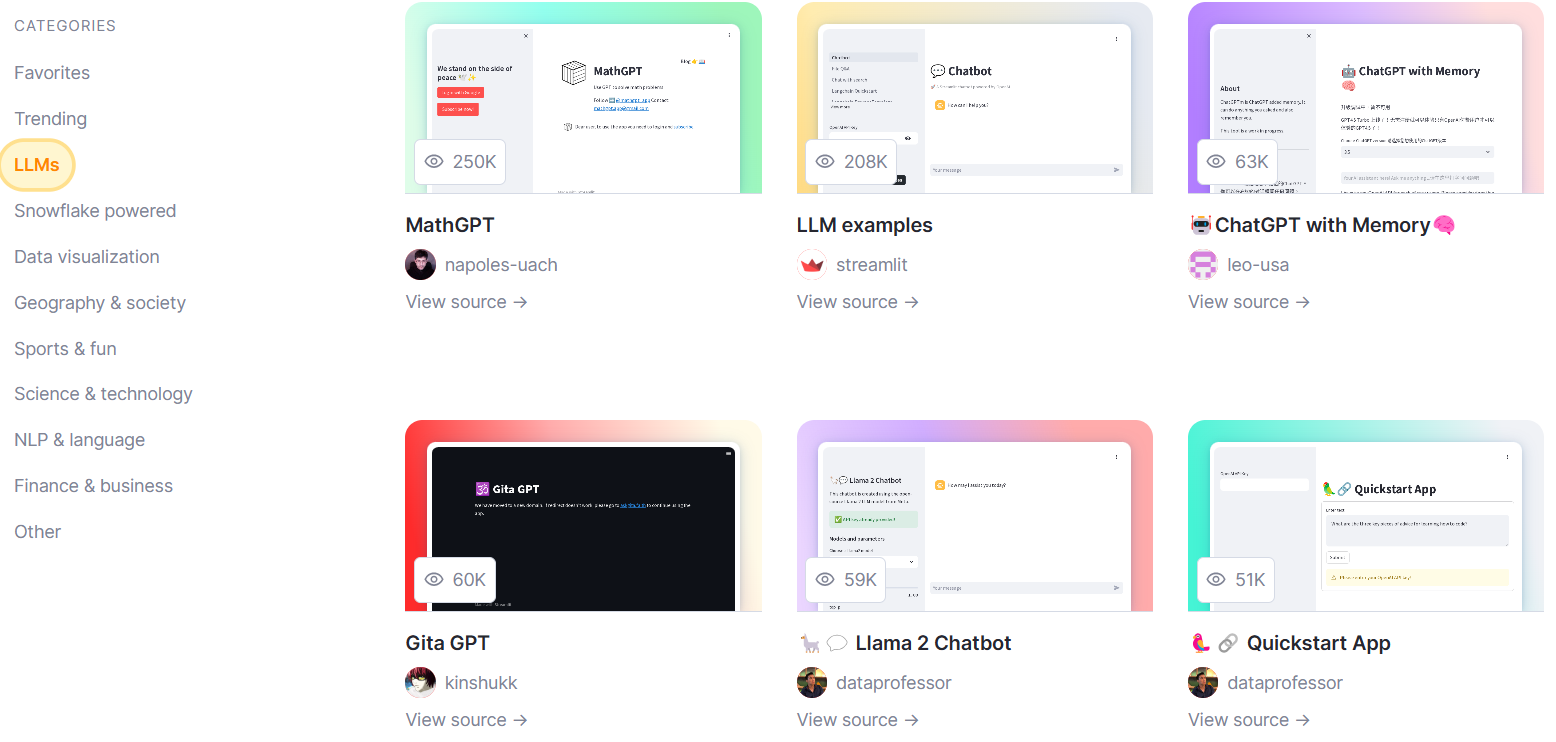
\includegraphics[width=\linewidth]{./figures/streamlit-app-gallery.png}
    \caption{Streamlit App Gallery.}
\end{figure}\newline

\subsubsection*{RAG pipelines development}
There are a few frameworks enabling developers to interact with LLMs and RAG pipelines, each of which provide different integrations with external APIs and tools: LangChain, LlamaIndex, Haystack, Langroid.\newline
The choice was made by 3S project coordinators to use LangChain for their solution. It is a great choice given that this platform provides all the tools to build complex RAG pipelines and personalize the different steps of these pipelines. Also, since its emergence in October 2022, this library has gained remarkable prominence with courses available on DeepLearning.ai, tutorials from NVIDIA, OpenAI, Google and others in addition to the exhaustive documentation available online.
\begin{figure}[htbp]
    \centering
    
\includegraphics[width=.5\linewidth]{./figures/langchain-logo.png}
    \caption{LangChain logo}
\end{figure}\newline
This framework has all the required components to build the most advanced RAG pipelines: Data loading from various sources, LLM and vector store integrations from different providers (both locally and on the cloud), prompt templates for different LLMs and tasks, etc...
\begin{figure}[htbp]
    \centering
    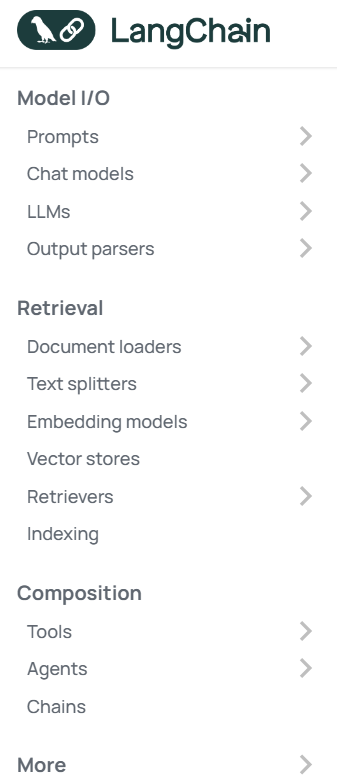
\includegraphics[width=.45\linewidth]{./figures/langchain-components.png}
    \caption{LangChain Components. (\href{https://python.langchain.com/v0.1/docs/modules/}{LangChain Documentation})}
\end{figure}\newpage

\subsection{LLMs}
There is a plethora of models of this type, both closed and open source, with many ways to access and use them.
\subsubsection*{Locally through Hugging Face Hub}
Many open-source LLM variants are available on Hugging Face Models Hub, as it is the main developer of the 'transformers' Python library.
\begin{figure}[htbp]
    \centering
    
\includegraphics[width=0.4\linewidth]{./figures/hf-logo.png}
    \caption{Hugging Face logo. \href{https://huggingface.co/models}{[Hugging Face models Hub]}}
\end{figure}
\begin{quote}
    "The Hugging Face Hub hosts many models for a \href{https://huggingface.co/tasks}{variety of machine learning tasks}. Models are stored in repositories, so they benefit from \href{https://huggingface.co/docs/hub/repositories}{all the features} possessed by every repo on the Hugging Face Hub. Additionally, model repos have attributes that make exploring and using models as easy as possible."  (\href{https://huggingface.co/docs/hub/models}{[Hugging Face Models Hub documentation]}, 2024)
\end{quote}
We can find an abundance of pre-trained LLMs downloadable from the HF Hub.
\begin{figure}[htbp]
    \centering
    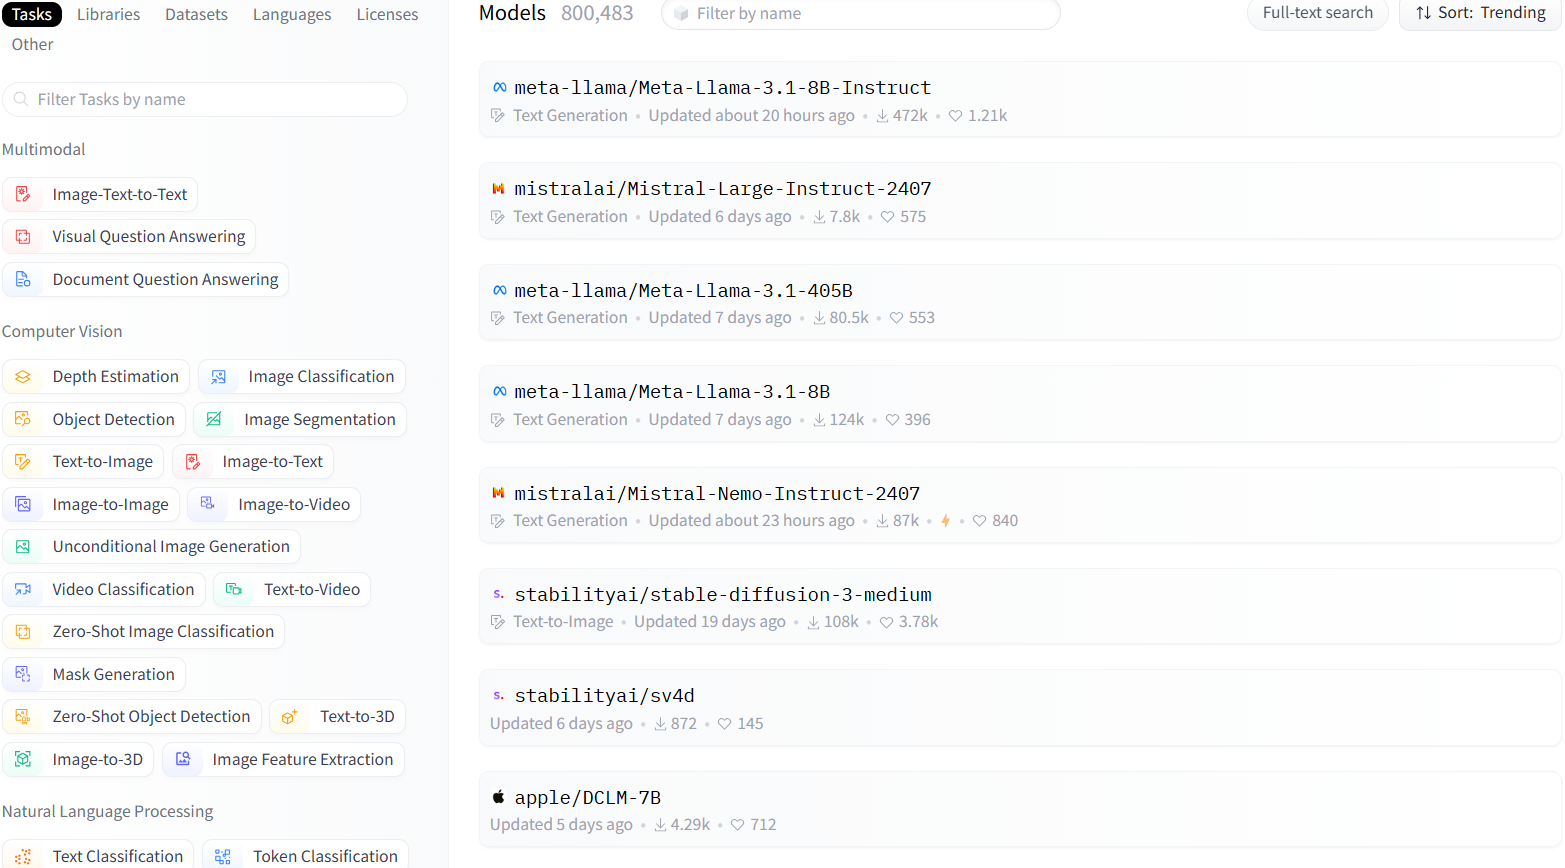
\includegraphics[width=.85\linewidth]{./figures/hf-models.png}
    \caption{A short list of popular models hosted on HF Hub, which can be explored by their categories/tasks. \href{https://huggingface.co/models}{[Models - Hugging Face]}}
\end{figure}\newline
This method allows the free utilization of a pre-trained model without being confined to cloud-platforms and their plans. As discussed in the previous chapter, this method will be used for the embedding model.
\begin{figure}[htbp]
    \centering
    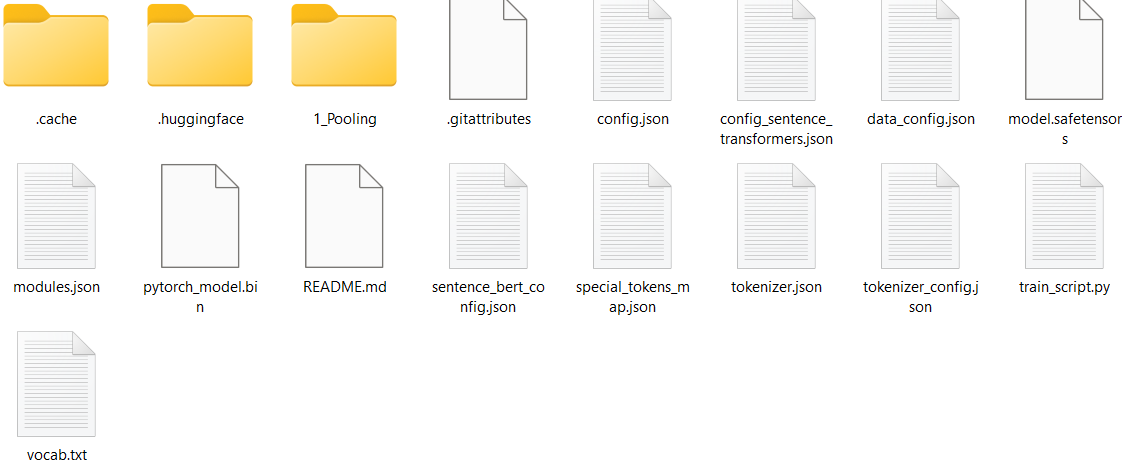
\includegraphics[width=\linewidth]{./figures/mpnet-local-files.png}
    \caption{The contents of a model repository downloaded locally \href{https://huggingface.co/sentence-transformers/all-mpnet-base-v2}{(all-mpnet-base-v2) on Hugging Face Hub}}.
\end{figure}\newline

\subsubsection*{API-enabled services and Cloud-based solutions}
Many companies behind Large Language Models development provide APIs or cloud-based environments to access their models. Some of the most popular options include OpenAI API, Google Cloud Vertex AI, Anthropic, Cohere, FireworksAI, MistralAI, TogetherAI, GroqCloud among others.\newline
This method, in contrast to running models locally, does not come with the pre-requisites of expensive hardware or delayed answer generation. Even though these solutions are paid services, most provide free trials and some of the available free plans only has a limit on daily and monthly usage, and is usually enough for personal usage. In addition to this, some of these cloud environments provide many models to use. For instance, FireworksAI allows to use Llama-3, Yi-Large, Mixtral, while TogetherAI provides models such as Qwen-2, Gemma (open-source version of Google's model, Gemini), Phi-2, Nous Capybara, and many others, all from within a single platform.
\begin{figure}[htbp]
    \centering
    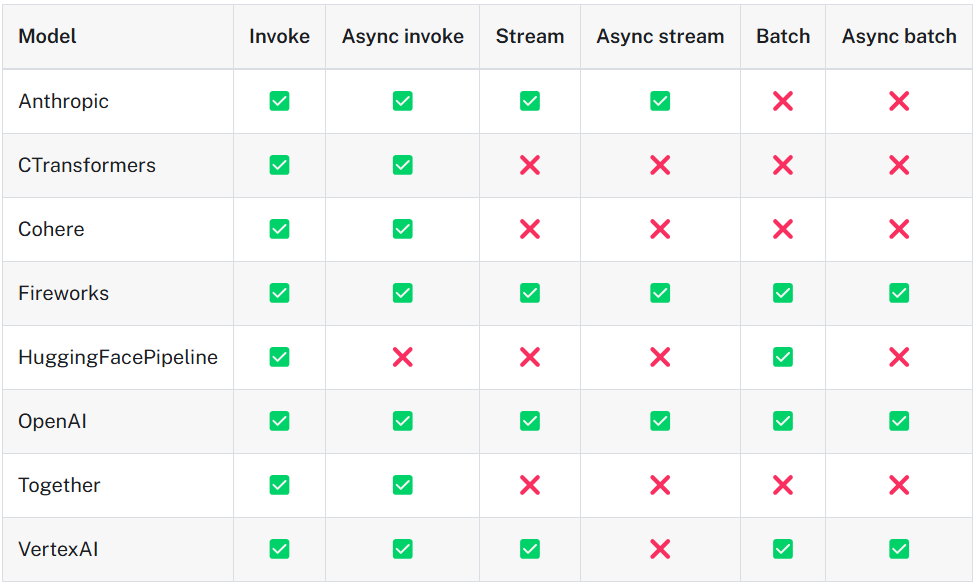
\includegraphics[width=\linewidth]{./figures/langchain-llm-integrations.png}
    \caption{LangChain Integrations with LLMs cloud providers. \href{https://python.langchain.com/v0.1/docs/integrations/llms/}{[Langchain Documentation - LLMs]}}
    \begin{flushleft}
        \small The previous list presents a subset of the integrations provided by Langchain. In addition to the aforementioned items, MistralAI and GrokCloud were integrated in the system to provide a plethora of Large Language Models suitable for Retrieval-augmented Generation. This solution also allows for some customization options through their web interfaces and API function parameters, even though limited when compared to local implementation.
    \end{flushleft}
\end{figure}
\begin{figure}[htbp]
    \centering
    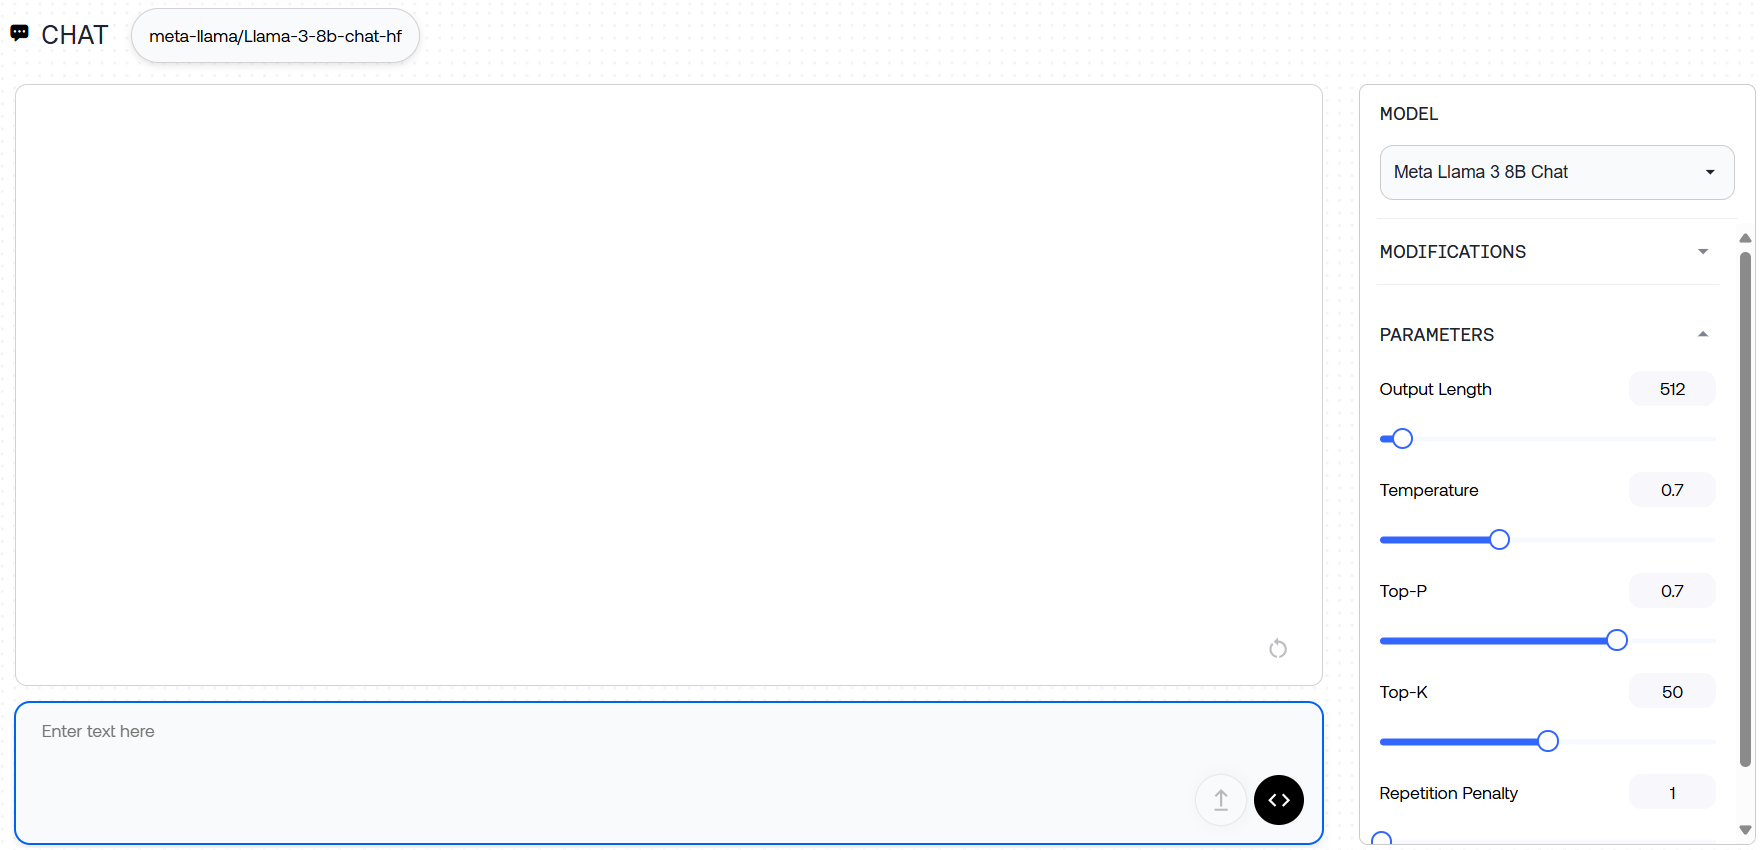
\includegraphics[width=\linewidth]{./figures/togetherai-playground.png}
    \caption{TogetherAI playground web interface, an example of a cloud-based environment allowing multiple LLM's customization options and parameters. \href{https://api.together.ai/playground}{TogetherAI Playground service}}
\end{figure}
\newpage

\subsection{Vector Stores}
There are many vector stores and embedding models to choose from which we will look through their differences.\newline
The choice of the most suitable vector store solution was based on four criteria mainly:
\begin{itemize}
    \item Self-hosting: This means that the vector store will be managed locally on the same computing infrastructure as the web server. This is opposed to a cloud-based deployment, which comes with the drawbacks of higher latency, possible network errors and high-costs.
    \item Latency: This refers to the performance and speed of similarity searching algorithms which are provided by the vector store and its ability to index and handle large volumes of data with the utilization of GPU parallel computing features.
    \item Accuracy: The relevance of retrieved data to the actual searched query. Often, this has a reverse relation with latency, as more accurate results take longer to be achieved.
    \item Documentation: Online Documentation and community forums that can guide on how to use the database efficiently.
\end{itemize}
\begin{table}[htbp]
    \begin{tabular}{|c|c|c|c|c|}
        \hline
        \textbf{\textcolor{darkgray}{Vector Store}} & \textbf{\textcolor{darkgray}{Self-hosting}}               & \textbf{\textcolor{darkgray}{Latency}} & \textbf{\textcolor{darkgray}{Accuracy}} & \textbf{\textcolor{darkgray}{Documentation}} \\  \hline
        \textbf{FAISS}                              & \textcolor{green}{\ding{52}}                              & \textcolor{green}{\ding{52}}           & \textcolor{green}{\ding{52}}            & \textcolor{red}{\ding{56}}                   \\ \hline
        \textbf{Pinceone}                           & \textcolor{red}{\ding{56}}                                & \textcolor{green}{\ding{52}}           & \textcolor{red}{\ding{56}}              & \textcolor{green}{\ding{52}}                 \\ \hline
        \textbf{Chroma}                             & \textcolor{green}{\ding{52}} / \textcolor{red}{\ding{56}} & \textcolor{green}{\ding{52}}           & \textcolor{red}{\ding{56}}              & \textcolor{green}{\ding{52}}                 \\ \hline
        \textbf{Lance}                              & \textcolor{green}{\ding{52}}                              & \textcolor{red}{\ding{56}}             & \textcolor{red}{\ding{56}}              & \textcolor{red}{\ding{56}}                   \\ \hline
    \end{tabular}
    \caption{Comparison of popular vector databases}
\end{table}\newpage
After careful consideration, FAISS vector store was selected due to its high performance and accuracy in comparison to alternatives. It leverages the GPU-enabled CUDA toolkit, and provides a state-of-the-art implementation of similarity searching algorithms based on this structure.
\begin{figure}[htbp]
    \centering
    
\includegraphics[width=\linewidth]{./figures/faiss_logo.png}
    \caption{FAISS logo.}
\end{figure}\newline
\begin{quote}
    FAISS is a FOSS library, it stands for "Facebook AI Similarity Search" with an implementation of nearest-neighbor search and k-selection algorithms designed specifically to efficiently handle large data sets, 8.5x faster than previous methods.
\end{quote}

\subsection{Embedding Model}
We have the choice to select the most suitable embeddings model.\newline
We have highlighted in the second chapter the importance of an embedding algorithm that minimize the loss of semantics when converting textual data to embedding vectors. In addition to this, considering that a vector store once initiated with an embedding model, can no longer swap it with another (unless re-initialized from zero). For this purpose, it would be a bad choice to consider cloud solutions as these may be unavailable in some cases (network or provider failure, expiration of tokens...).\newline
The best choice in this case, as in vector store's choice, is to select a suitable model which is available offline (as in self-hosting). This will avoid foreseeable failures and limit problems.\newline
This redirects us to the Hugging Face Hub where we can find many embedding models, which are available through the sentence transformers-repository.
\begin{figure}[htbp]
    \centering
    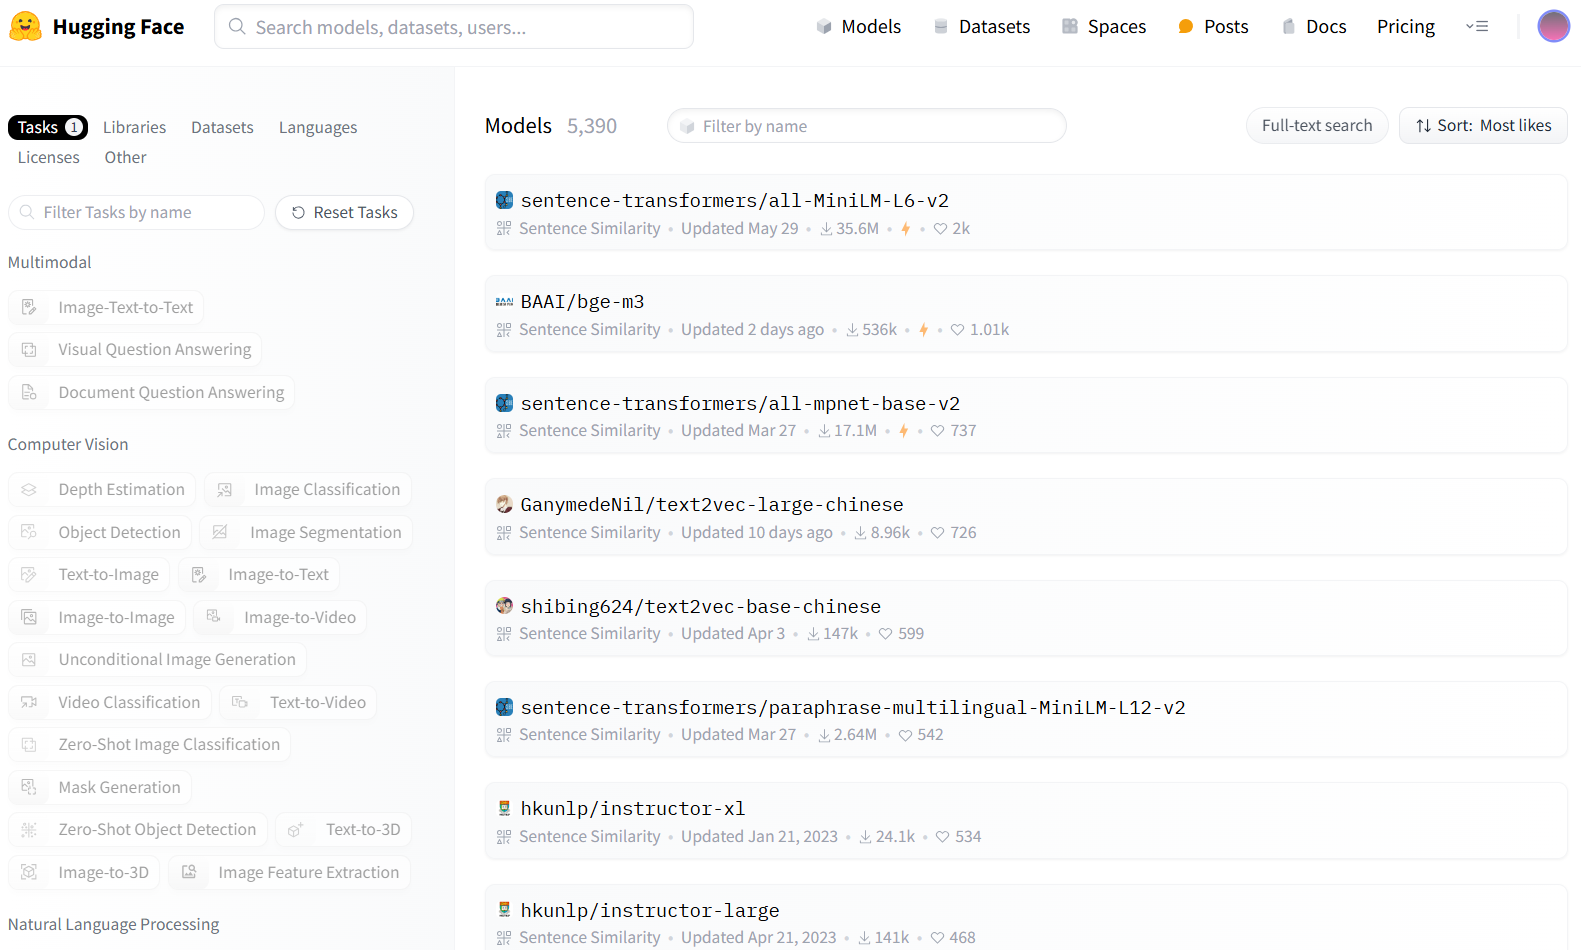
\includegraphics[width=.85\linewidth]{./figures/hf-embedding-models.png}
    \caption{A short list of popular embedding models available on HF Hub. \href{https://huggingface.co/models?pipeline_tag=sentence-similarity&sort=likes}{HF models filtered by `sentence-similarity` task}}
\end{figure}\newline
Two of the most popular choices are "all-MiniLM-L12-v2" and "all-mpnet-base-v2", the first of which makes a better choice when working in a limited environment while not paying much attention to retaining semantics (faster embedding generation and smaller size), while the second one, "all-mpnet-base-v2", is the more suitable choice for our case due to, even with its larger footprint, its capability to capture most of the semantics and meanings of sentences.\newpage
\begin{figure}[htbp]
    \centering
    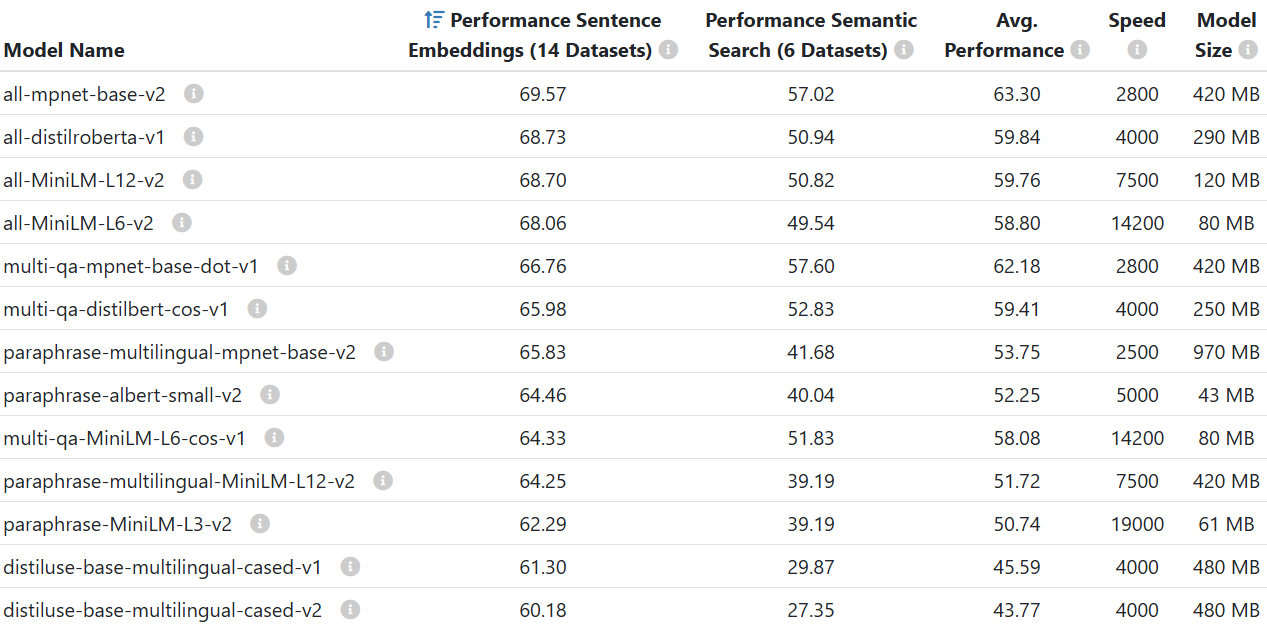
\includegraphics[width=\linewidth]{./figures/embedding-modes-performance.png}
    \caption{Sentence-Tansformers model performance comparison \href{https://sbert.net/docs/sentence_transformer/pretrained_models.html}{[Pre-Trained Sentence Transformers models' performance]}}
\end{figure}
\begin{quote}
    "The all-* models were trained on all available training data (more than 1 billion training pairs) and are designed as general purpose models. The all-mpnet-base-v2 model provides the best quality, while all-MiniLM-L6-v2 is 5 times faster and still offers good quality."  (\href{https://sbert.net/docs/sentence_transformer/pretrained_models.html}{[Sentence Transformers documentation]})
\end{quote}
\newpage

\section{Incorporating into a functional RAG system}
After introducing the frameworks and tools which would allow us to build a RAG system, it is necessary to discuss the implementation details of these elements and how they were incorporated together.\newline
This section is dedicated to showcasing how these components interact together in the implemented solution.
\begin{figure}[htbp]
    \centering
    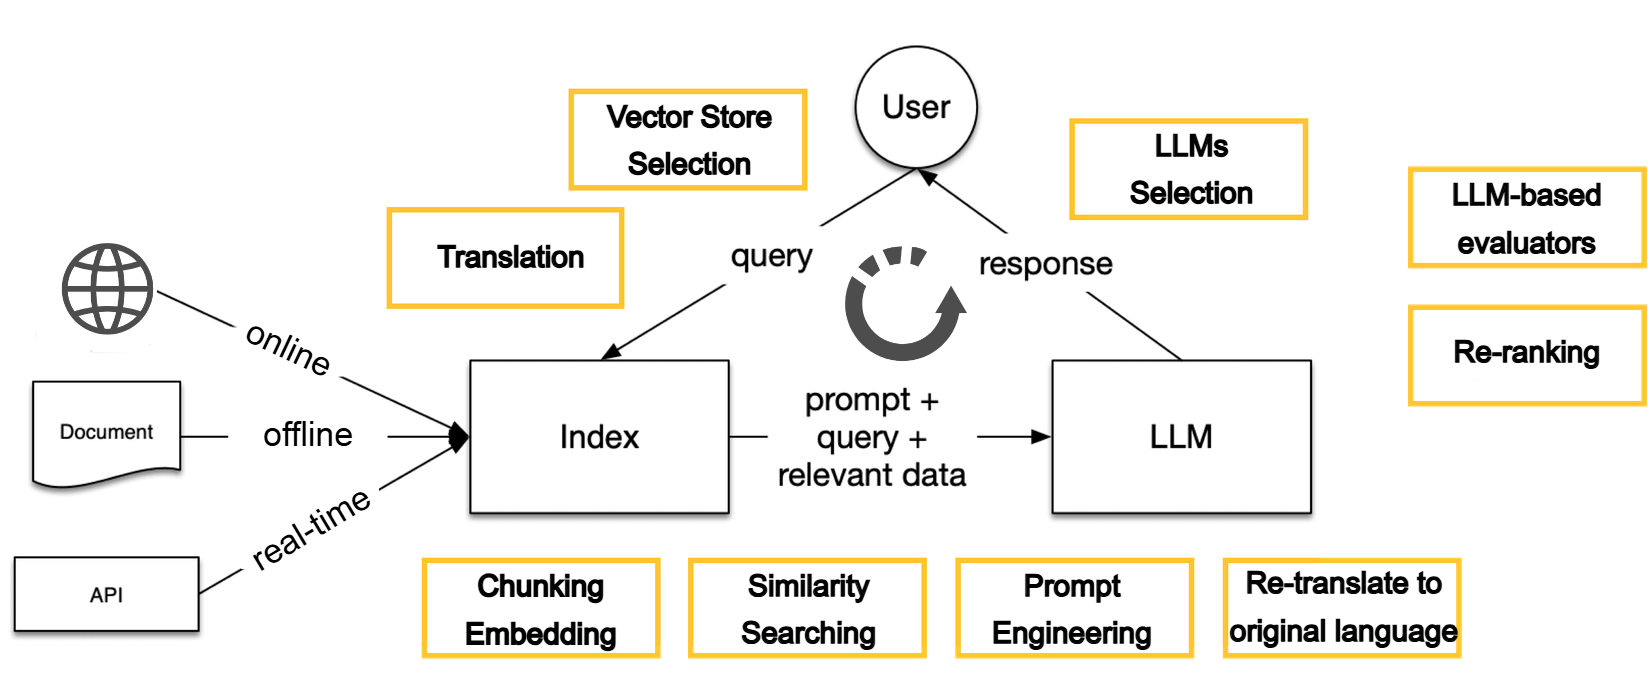
\includegraphics[width=\linewidth]{./figures/rag_components.png}
    \caption{The overall pipeline of the system to be implemented, showcasing the interaction between the different components, from knowledge augmentation methods (document/data loading and chunking etc...), vector database (index), RAG pipeline (User-Index-LLM interaction), re-ranking and evaluation processes}
\end{figure}\newline
This figure demonstrates the overall process that are executed in the system:
\begin{itemize}
    \item Loading data from online web content, offline documents and files, or real-time data from APIs (Search engines and GPT Researcher) after which the chunking and embedding transformation occur.
    \item User preference selections (vector stores, LLMs, enable translation or not)
    \item Typical RAG processes: retrieval (similarity searching), prompt engineering and transformation, and finally generation
    \item Reiterate the RAG pipeline for every LLM selection (automatically retranslate the answer to the user's language if needed).
    \item Re-Ranking of answers based on RAG metrics and user feedback.
\end{itemize}
\newpage

\subsection{Data Ingestion Methods}
The first essential part of the project is to allow the on-demand ingestion of data and new information into the vector store.\newline
For this purpose, various file formats and online web scraping and fetching methods have been implemented; LangChain, as seen in the previous section, provides a "Document loaders" section in its "Retrieval" toolbox. These tools provide many tutorials and helpful functions to implement document loading and chunking from various sources, which has allowed to accomplish the required methods to satisfy the coordinating teams at 3S.
\begin{figure}[htbp]
    \centering
    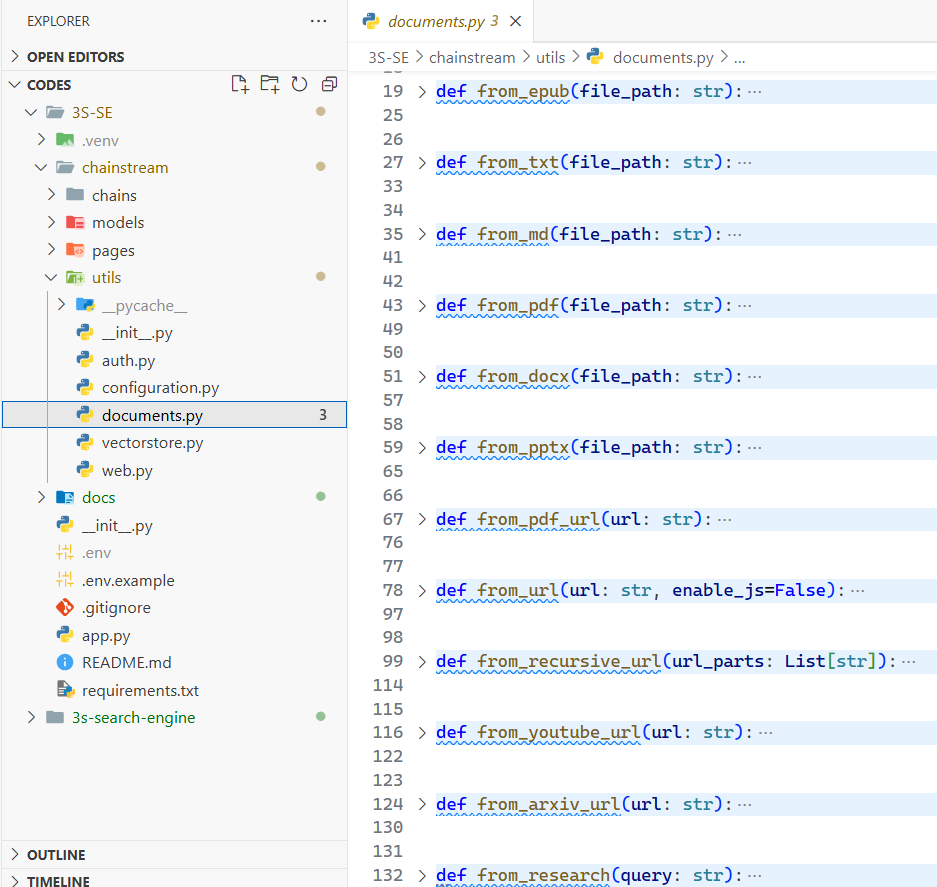
\includegraphics[width=\linewidth]{./figures/data-ingestion-methods.png}
    \caption{Various data ingestion methods}
\end{figure}\newline
To make it more comprehensible, here is a short description of what each of these methods do:
\begin{itemize}
    \item Web Pages (from\_url, from\_recursive\_url): Allowing to read a single page from a given URL, or a page and its child pages recursively, supporting static and dynamic web content.
    \item Arxiv Research Papers (from\_arxiv\_url): Allows to read content directly from an arxiv URL, conserving metadata like author, dates, etc...
    \item Youtube Content (from\_youtube\_url): Transcribes a video uploaded on YouTube and constructs a document from a given URL.
    \item Generative Research (from\_research): Utilizes \href{https://gptr.dev/}{GPT Researcher}, a tool that allows to, given a question, generate multiple queries to send to search engines and then generating an artificial report.
    \item EPUB files (from\_epub): This is an e\-book format suitable for storing and distributing large volumes of information.
    \item Text files (from\_txt): A file format for storing texts and notes.
    \item Markdown files (from\_md): An easy to use syntax to write documentation and notes
    \item PDF files (from\_pdf): Allowing to read PDF files.
    \item Same for other file formats...
\end{itemize}
Toolkits: NLTK, BeautifulSoup, Playwright, Unstructured, PyMuPDF, Pandoc, GPT Researcher, Tavily, LLMs

\subsection{Retrieval}
\subsubsection{Vector Store}
As outlined in the project objectives, the implementation of a vector database should allow different teams to upload their documents into separate vector databases.\newline
To achieve this, two Python classes have been implemented: one to hold the vector store functionalities: loading and saving to local storage in addition to listing available databases, and another to manage access credentials to vector store through a name and a passphrase.
\begin{figure}[htbp]
    \centering
    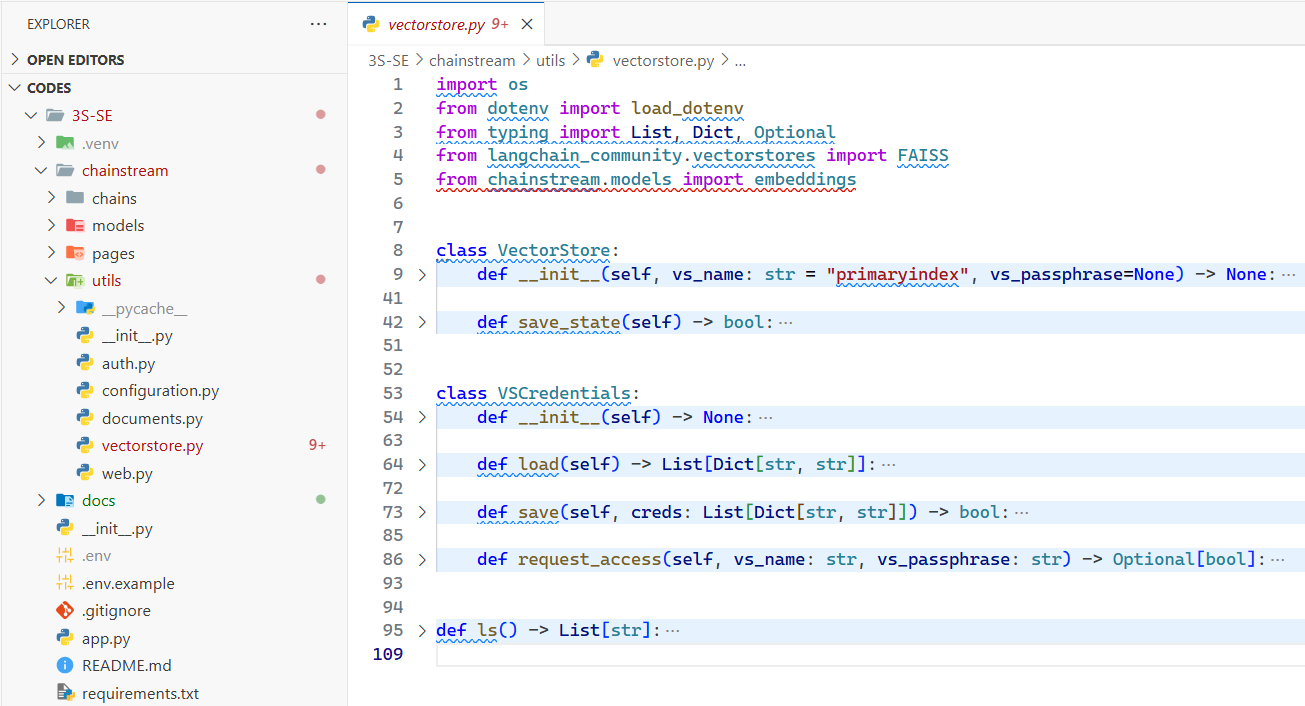
\includegraphics[width=\linewidth]{./figures/vectorstore-implementation.png}
    \caption{Vector Store implementation classes and methods}
\end{figure}\newline
A vector store can be initialized with "vs\_name" alone, which gives the read access to its contents. To modify it however, one should provide it with a passphrase ("vs\_passphrase"), which would give users who have gained access the ability to load new content through the various data ingestion methods previously mentioned.\newpage
\begin{figure}[htbp]
    \centering
    
\includegraphics[width=.8\linewidth]{./figures/vectorstore-local-dir.png}
    \caption{Local Directory for storing vector stores.}
\end{figure}
The "creds.json" file store access credentials to the available vector stores, while other folders ("3S" and "SSS" in this example) holds the vector store's data.
\subsubsection{Chunking and Embedding}
A vector store initialization typically includes an embedding model initialization, which vectorizes the documents' chunks. For our case, as we chose to select a model from Hugging Face Hub ("all-mpnet-base-v2"), we need to ensure that the model is downloaded and stays up-to-date.
\begin{figure}[htbp]
    \centering
    \begin{subfigure}{0.45\textwidth}
        \centering
        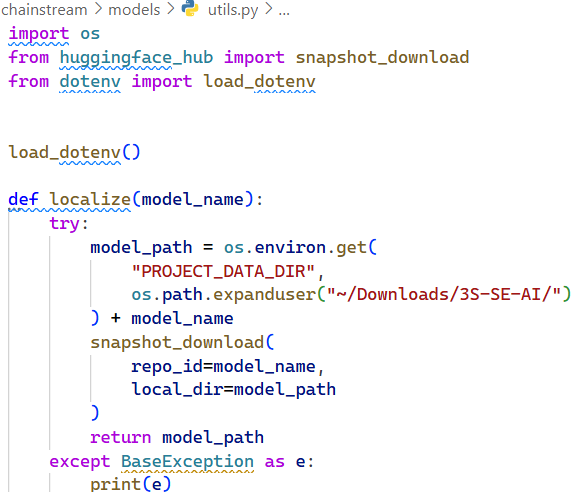
\includegraphics[width=\linewidth]{./figures/embedding-model-downloading.png}
        \caption{Downloading}
    \end{subfigure}
    \hfill
    \begin{subfigure}{0.45\textwidth}
        \centering
        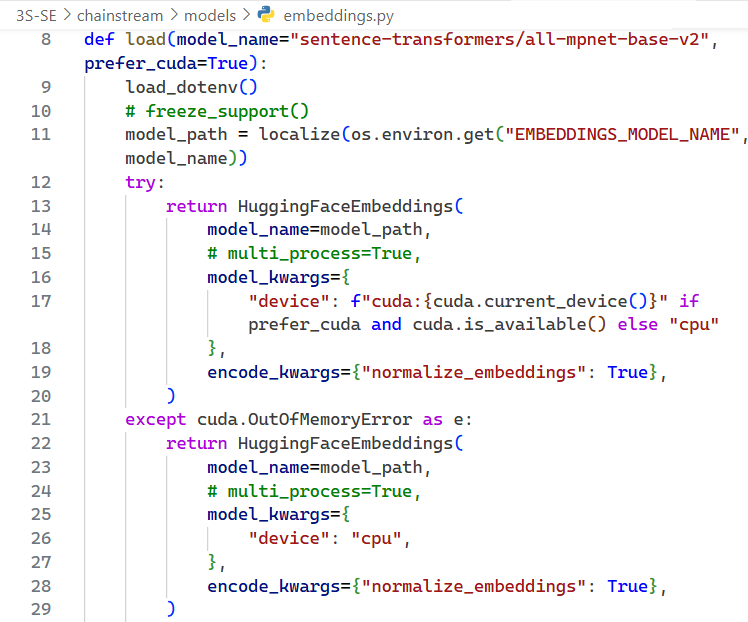
\includegraphics[width=\linewidth]{./figures/embedding-model-loading.png}
        \caption{Loading}
    \end{subfigure}
    \caption{Embedding Model Implementation}
\end{figure}\newline
The "snapshot\_download" function imported from "huggingface\_hub" ensures that the latest version of the model is available locally and can be loaded, while the implemented `load` function leverages it by loading the model on the GPU and falls back to the CPU when needed.\newpage
\subsubsection{Retrieval and Similarity Search}
In some cases where the knowledge base does not contain relevant information to the user query, naive RAG would retrieve the passages with the highest similarity score, even if its contents are not pertinent to the question. This issue is addressed by only including documents which scores attain a certain threshold, eliminating unnecessary passages thus reducing context size when prompting LLMs, and providing trustworthiness when no content can be found so the LLMs inform the user rather than introducing hallucination in generated answers.
\begin{figure}[htbp]
    \centering
    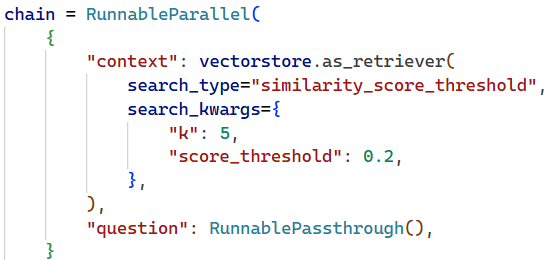
\includegraphics[width=\linewidth]{./figures/similarity_search_threshold.png}
    \caption{Similarity Search Tuning}
    \begin{flushleft}
        \small The score\_threshold parameter allows to set a value which only passage that has a higher score are passed to the LLM's context, eliminating irrelevant information and setting a limit on the maximum number of passages (k parameter set to 5). The choice of these values was based on experimentation and testing with different values, where some relevant information could be dismissed if the threshold was set to a higher value, and the risk of irrelevancy was significant if set to lower value.
    \end{flushleft}
\end{figure}\newline

\subsection{LLMs and Prompts}
As new products and cloud platforms are constantly emerging and changing rapidly, the models and tools (web searching APIs), which allow the LLMs to connect to external web searching APIs, were implemented in an extendible manner, where adding, removing or customizing LLMs and their behavior is an easy change in code. The following code snippet showcases the tool loading process when the environment is started.
\begin{figure}[htbp]
    \centering
    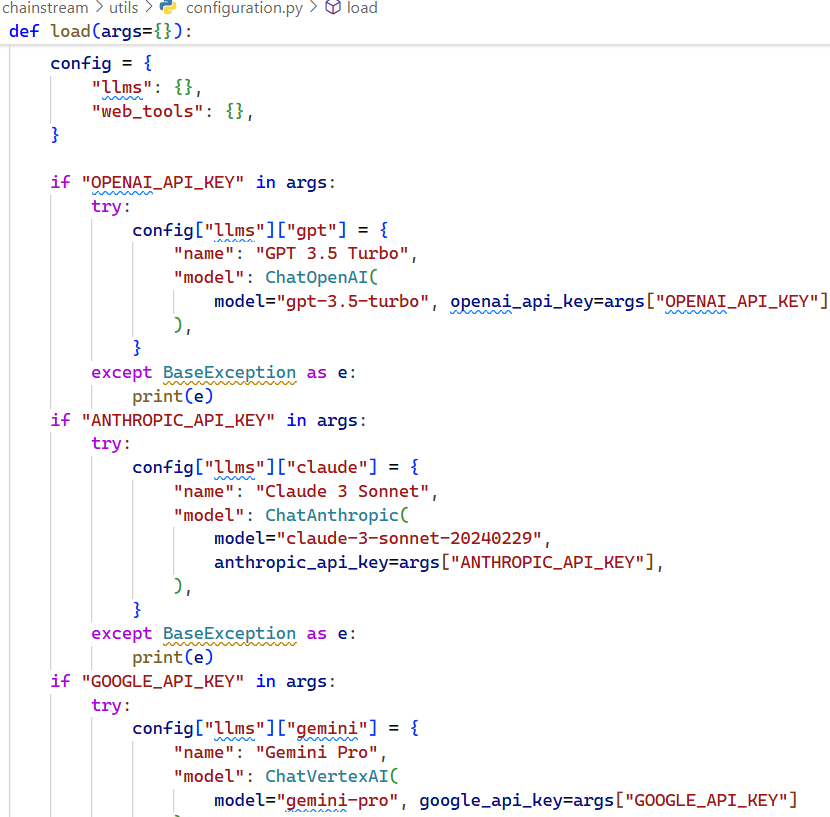
\includegraphics[width=.9\linewidth]{./figures/llms-implementation.png}
    \caption{Implementation of LLMs and Prompts, focusing on extensibility}
    \begin{flushleft}
        \small The lists of Large Language Models ("llms" key in the "config" variable) and tools ("web\_tools") grow dynamically when provided with valid API keys.
    \end{flushleft}
\end{figure}\newline
The list is much longer than this illustration, still it is easy to figure out how to add other LLMs and APIs as needed.\newline
In addition to these APIs, this loading mechanism allows for flexible Prompt modification when different models require different prompts.\newpage
\begin{figure}[htbp]
    \centering
    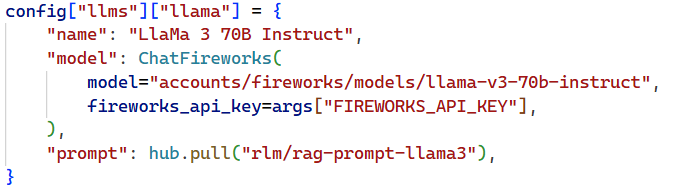
\includegraphics[width=\linewidth]{./figures/prompt-template-impl.png}
    \caption{Incorporating prompts into model definition.}
\end{figure}
This approach allows to define a custom prompt template suitable for a specific model (such as in our case of Llama 3) from within a unified source code file. In theory, the "prompt" field can hold any f-string format (a concept in Python used to interpolate variables dynamically into a string), but the \href{https://smith.langchain.com/hub}{LangChain Hub} provides many example prompts for different tasks.
\begin{figure}[htbp]
    \centering
    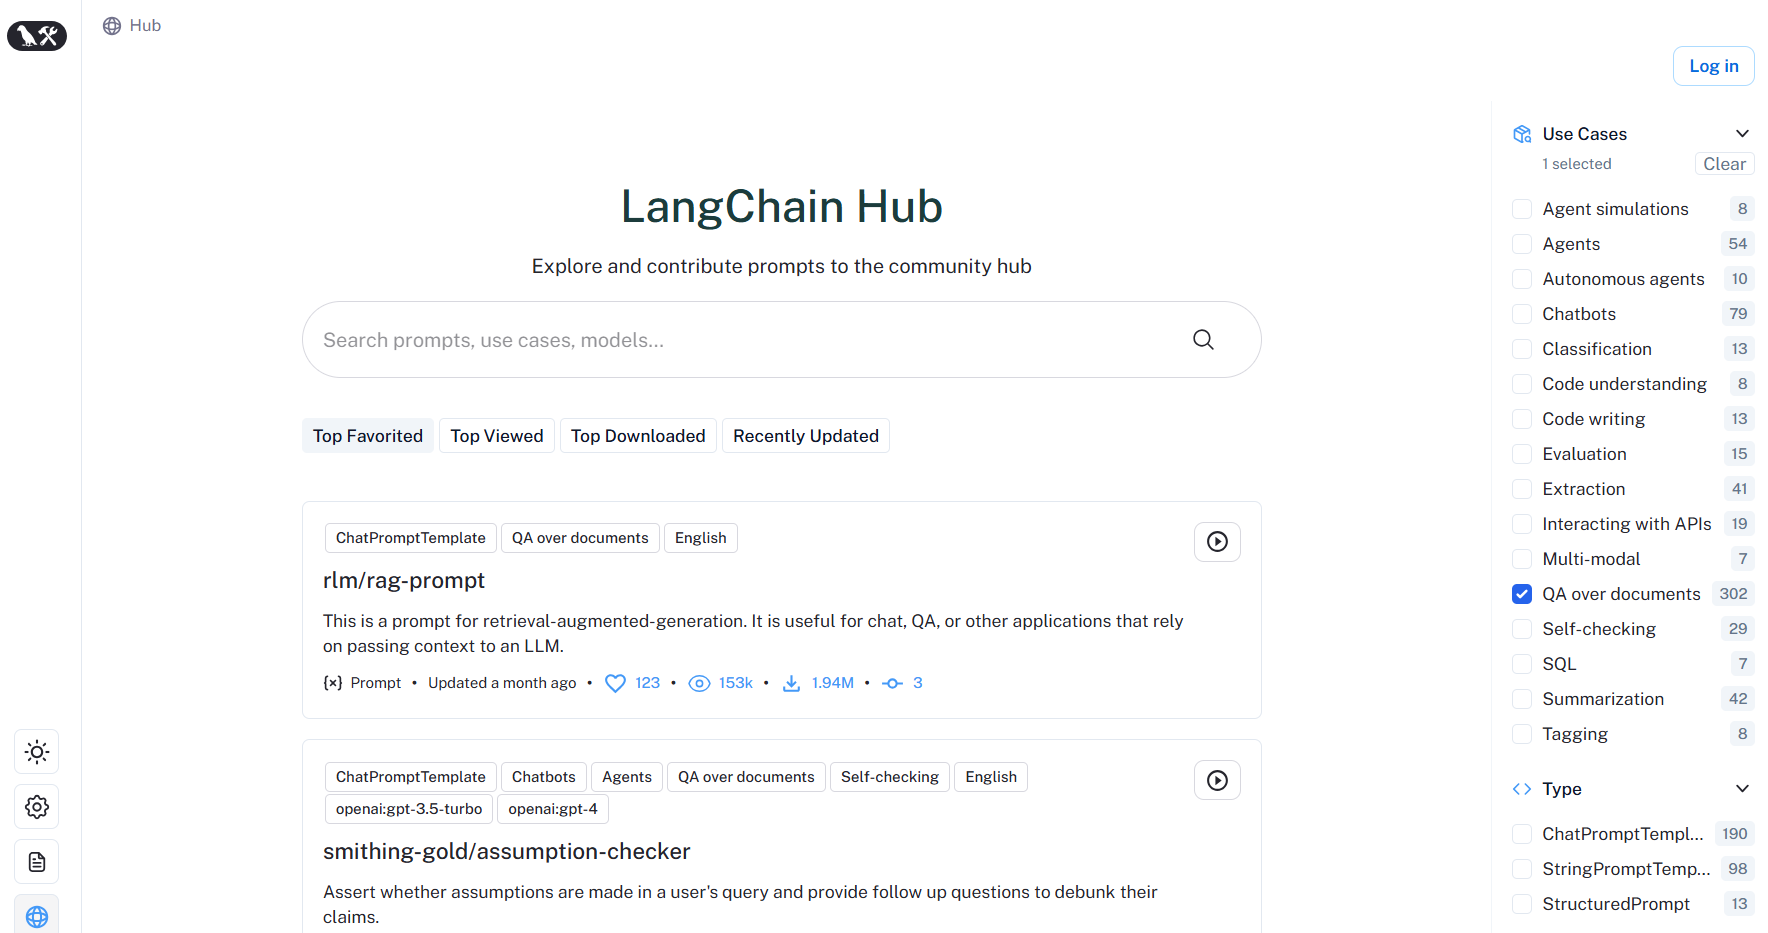
\includegraphics[width=\linewidth]{./figures/langchain-hub.png}
    \caption{LangChain Hub web interface.}
\end{figure}\newline
This Hub allows to find ready-to-use prompt templates suitable for various LLMs for Retrieval-augmented generation purposes.\medskip\newline
The resulting list of implemented LLMs is as follows.
\begin{figure}[htbp]
    \begin{subfigure}{\textwidth}
        \centering
        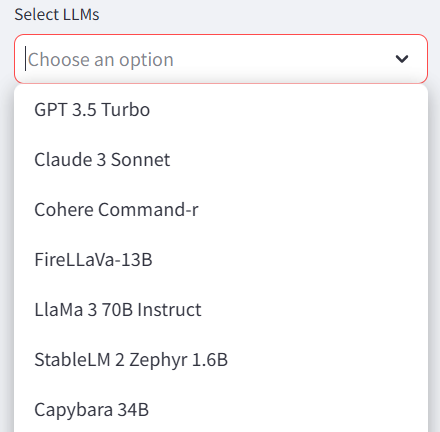
\includegraphics[width=.7\linewidth]{./figures/select-llms-p1.png}
    \end{subfigure}
    \begin{subfigure}{\textwidth}
        \centering
        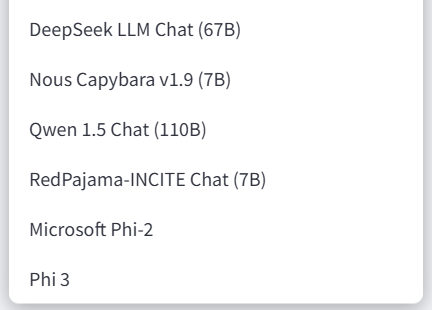
\includegraphics[width=.7\linewidth]{./figures/select-llms-p2.png}
    \end{subfigure}
    \caption{List of implemented LLMs}.
\end{figure}\newpage
\subsection{Evaluation and Ranking}
As multiple answer generations occur in parallel, it is essential to provide the better quality responses first. For this purpose, RAG-based metrics were implemented with the help of the Ragas library. It stands for Rag Assessment and provides various metrics to evaluate RAG pipeline performance.
\begin{figure}[htbp]
    \centering
    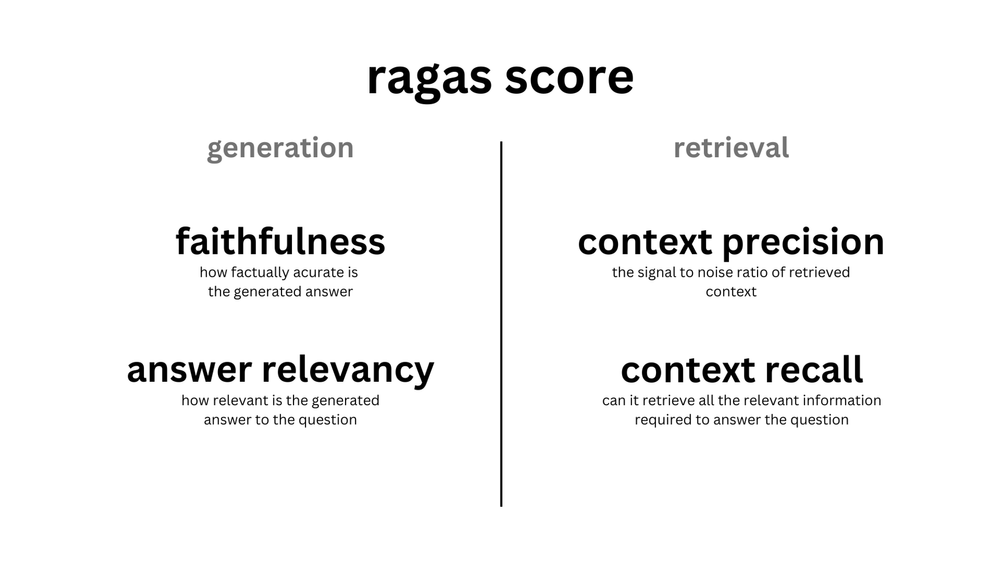
\includegraphics[width=\linewidth]{./figures/ragas-metrics.png}
    \caption{RAG pipeline evaluation metrics and description}
\end{figure}\newline
When combined with the similarity score returned by the vector store when retrieving documents, this library allowed to assess the retrieval phase context relevancy and generation phase consistency against the given context and the prompt.
In addition to these metrics, a user-driven feedback was implemented and integrated into the ranking algorithm to assess the overall satisfaction over a specific Large Language Model.
\begin{figure}[htbp]
    \centering
    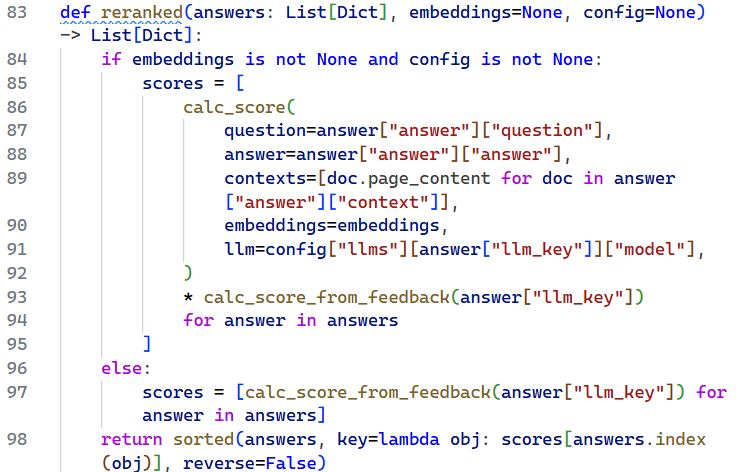
\includegraphics[width=\linewidth]{./figures/ranking-algo.png}
    \caption{Evaluation metrics for the ranking algorithm}
    \begin{flushleft}
        \small This function sorts the generated responses based on the evaluation scores it obtained. It calculates the score based on consistency of the generated answer against the given feedback and its relevancy against the question it received, in addition to the similarity score and the feedback given by users. The formula to calculate the score is as follows :
        score = feedback score * similarity score * faithfulness score * answer relevance score
    \end{flushleft}
\end{figure}\newline
\newpage

\section{Testing and Validation}
\subsection{Response without Retrieval-augmented Generation}
\begin{figure}[htbp]
    \centering
    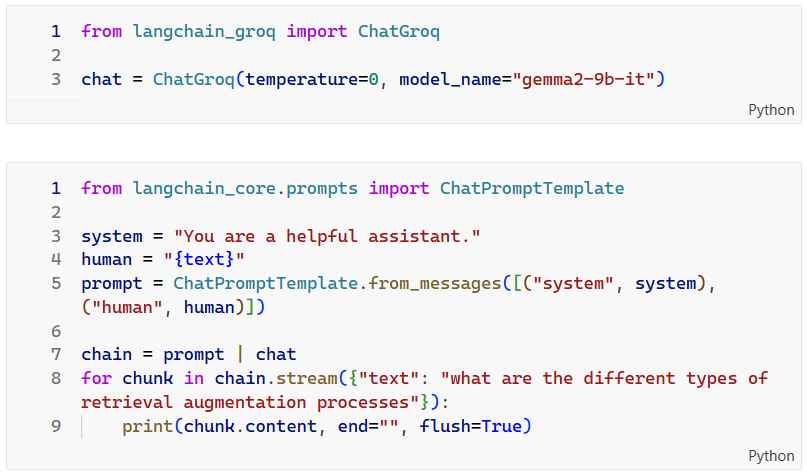
\includegraphics[width=\linewidth]{./figures/code-norag.png}
    \caption{Implementation of a Large Language Model (Gemma 2) without RAG functionality}
\end{figure}\newpage
The execution of the previous code resulted in the following output.
\begin{figure}[htbp]
    \centering
    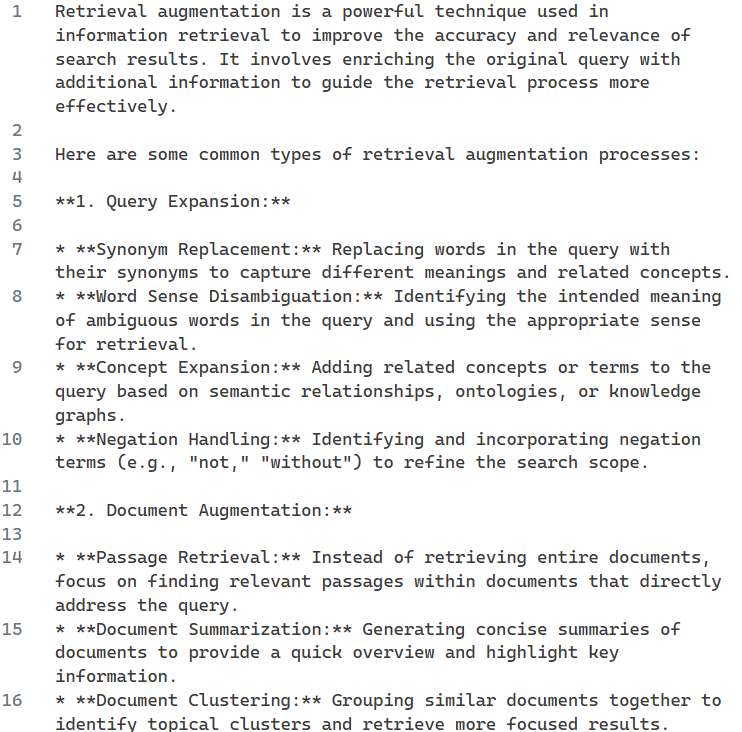
\includegraphics[width=\linewidth]{./figures/answer_norag.png}
    \caption{A Large Language model response without RAG}
\end{figure}\newline
The example demonstrates the inconvenience of using an LLM when looking for a short and accurate response to a given query ("what are the different types of retrieval augmentation processes"). The generated answer is very long and clearly exhibits hallucination, as it is not accurate enough.\newline
The next section is about how this inconvenience can be effectively rectified and changed to an acceptable behavior.\newpage
\subsection{Retrieval-augmented Generation results}
\subsubsection{Data: Question and Answer}
We will need to load some data into the knowledge base. This information represents the ground truth on which we desire LLMs to base their answers.\newline
For this purpose, a \href{https://arxiv.org/abs/2312.10997}{PDF file from a research parper on Arxiv} will be uploaded as target data. Page 11 of this document contain the answer to our previous question.
\begin{figure}[htbp]
    \centering
    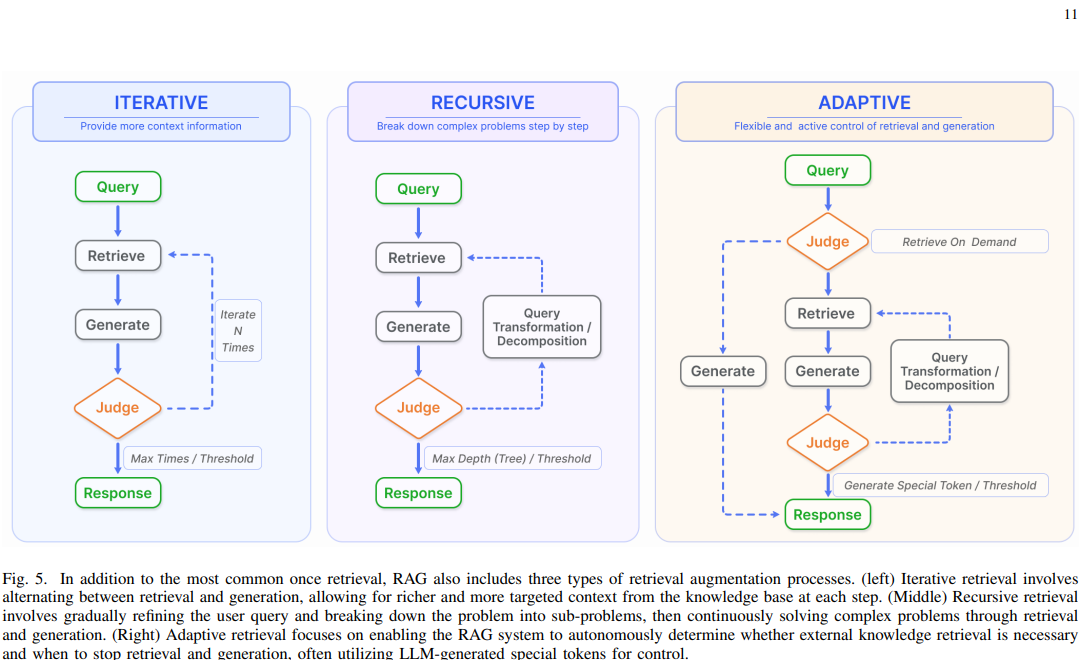
\includegraphics[width=\linewidth]{./figures/toberetrieved.png}
    \caption{The content of the document containing the desired answer to the question ("what are the different types of retrieval augmentation processes")}
    \begin{flushleft}
        \small This page from the PDF file contain clear answer to our question (3 types of retrieval augmentation processes: iterative, recursive, adaptive)
    \end{flushleft}
\end{figure}\newline
After having established a query to be asked to the model and its corresponding desired answer, we will now implement a simple RAG pipeline with the same previous model (Gemma 2) to see the difference in generated answers.\newpage
\subsubsection{Knowledge Base initialization}
The first step is to load the PDF file into the knowledge base. For this purpose, we need to initialize a FAISS index with an embedding model (all-mpnet-base-v2), which will convert the information read from the file through PyMyPDFLoader to a numerical representation suitable for similarity search afterwards.
\begin{figure}[htbp]
    \centering
    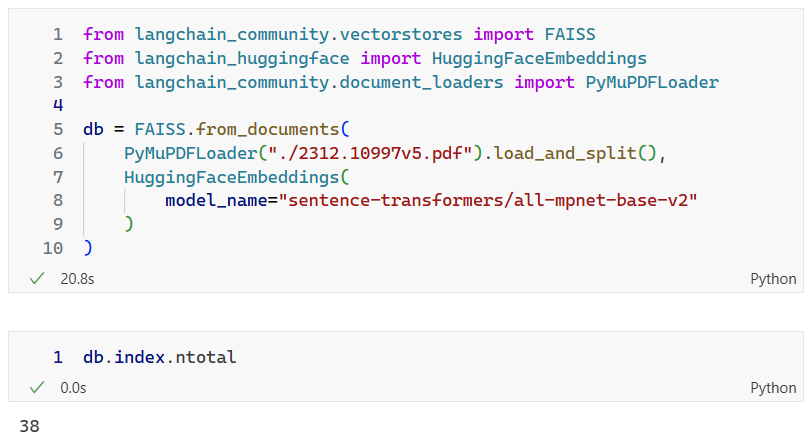
\includegraphics[width=\linewidth]{./figures/vectorstore_init.png}
    \caption{Vector Store initialization with data}
    \begin{flushleft}
        \small This sample vector store initialization included reading and loading the required PDF file from local storage, resulting in 38 chunks, which simplifies the process of retrieving and passing the most relevant chunks to the large language model later on.
    \end{flushleft}
\end{figure}\newpage
\subsubsection{Similarity Search dry run}
The following code imitates the retrieval phase in a complete RAG pipeline, providing an overview of the contents of the vector store and the results when some passages get retrieved.\newline
\begin{figure}[htbp]
    \centering
    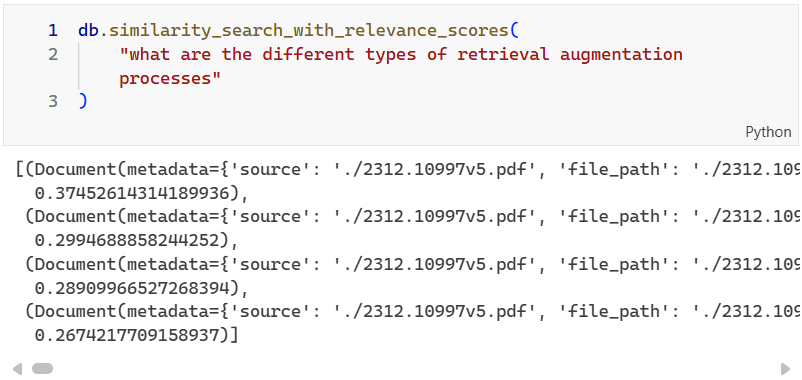
\includegraphics[width=\linewidth]{./figures/vectorstoresimilaritysearchwithscore_code.png}
    \caption{Retrieving relevant documents from the database}
\end{figure}
\begin{figure}[htbp]
    \centering
    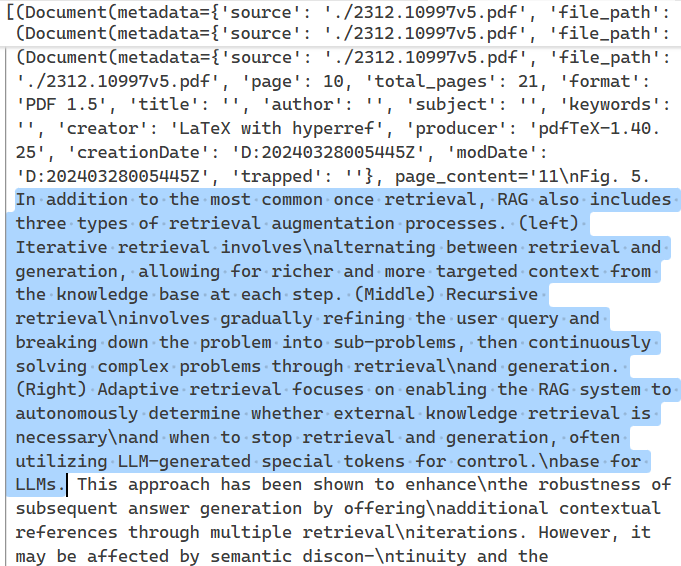
\includegraphics[width=\linewidth]{./figures/vectorstoresimilaritysearchwithscore_output.png}
    \caption{Output from similarity search}
    \begin{flushleft}
        \small The returned passages, as seen above, contain parsed text from the PDF file. As the vector store contain separate chunks, the result of running the previous code is a list containing document chunks, each with the textual content and some metadata that helps representing the whole documents through its chunks in a vector store. These chunks are sorted by their relevance score, which is calculated based on the cosine similarity measure between the query and the actual passage's embeddings vectors. The highlighted text is the desired data that we want to pass to the LLM afterwards. This passage is returned 3rd on the list, with a score of 0.28.
    \end{flushleft}
\end{figure}\newpage
The results of retrieval, even though still optimizable, is satisfactory. Given a query, it is almost impossible to not retrieve the relevant passage outside the first 5 elements. This is because of the indexing strategy implemented in the vector store which allows the calculation of the similarity between every chunk and the query to ensure most similar passages are retrieved effectively.\newline
These retrieved documents can now be integrated in a prompt and passed to the LLM to control the context of its generation process.\newpage
\subsubsection{Response with Retrieval-augmented Generation}
\begin{figure}[htbp]
    \centering
    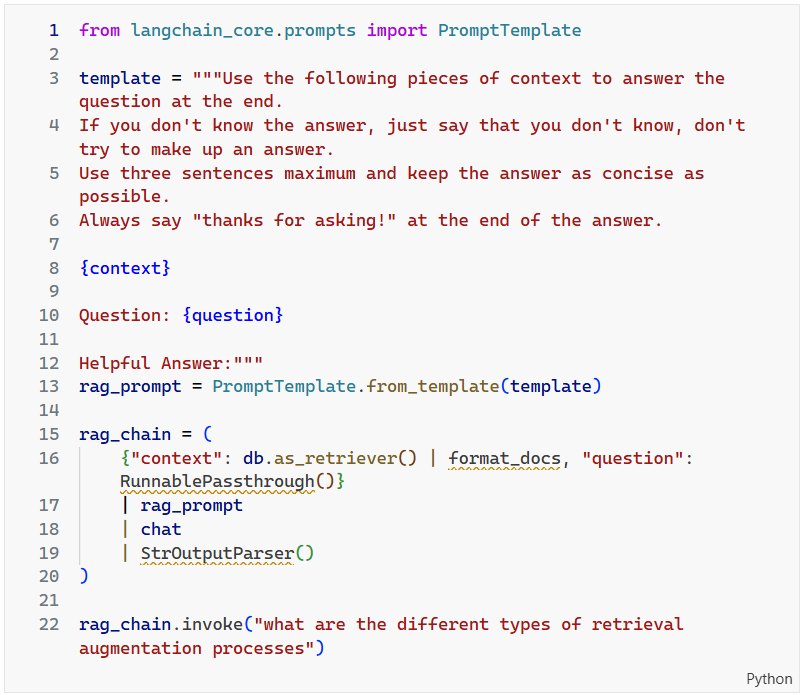
\includegraphics[width=.9\linewidth]{./figures/rag-code.png}
    \caption{Initialization of a simple RAG pipeline for testing}
    \begin{flushleft}
        \small The steps to initialize the RAG pipeline are: 1. set the prompt to support passing the context (retrieved documents) and question, along with instructing the model to only base its answer on the given context, 2. reconstructing the prompt by filling the variables (retrieving and formatting the context and the question), 3. passing the constructed prompt to the LLM (chat), 4. and finally transforming the LLM's response into a human readable format.
    \end{flushleft}
\end{figure}\newpage
Executing the previous code resulted in the desired output.
\begin{figure}[htbp]
    \centering
    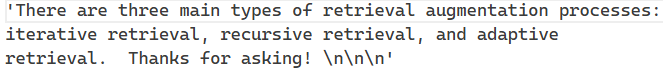
\includegraphics[width=\linewidth]{./figures/rag-answer.png}
    \caption{The generated answer from a RAG pipeline}
\end{figure}\newline
The response demonstrates how effective was the pipeline from transforming a long answer into a very accurate direct answer.
\subsection{RAG metrics sorting}
The sorting algorithm allows for better answers to be more accessible by placing them at the bottom of less accurate ones.
To showcase how it affects the results page, here is a comparison between the positioning of generated answers from four different models (Claude 3.5 Sonnet, Command R+, Gemma-2 and Llama-3), from the previous example's question.
\begin{figure}[htbp]
    \centering
    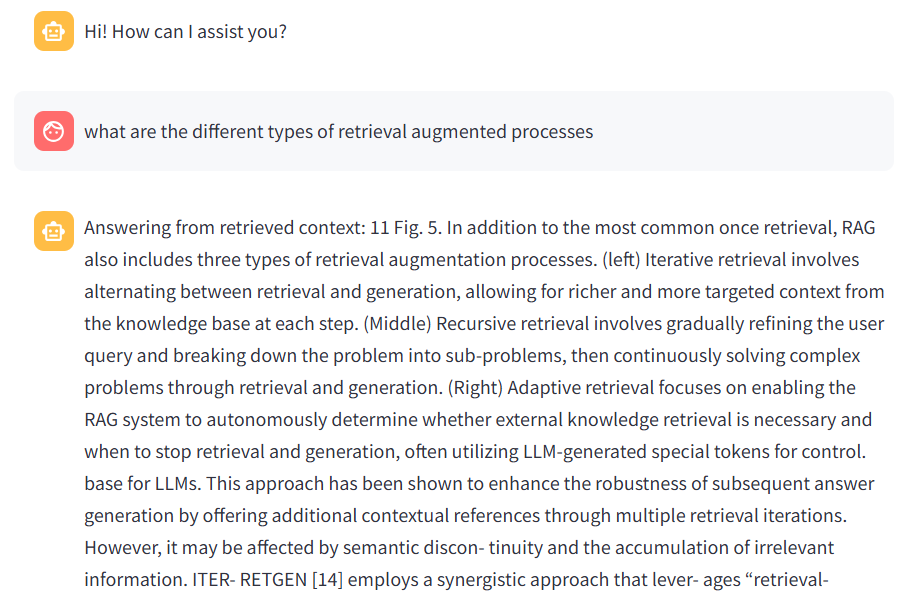
\includegraphics[width=\linewidth]{./figures/app-question.png}
    \caption{Prompting and retrieving context from the input question}
\end{figure}\newpage
After the context gets retrieved from the selected vector stores, the LLMs start generating answers based on its contents as shown below.
\begin{figure}[htbp]
    \centering
    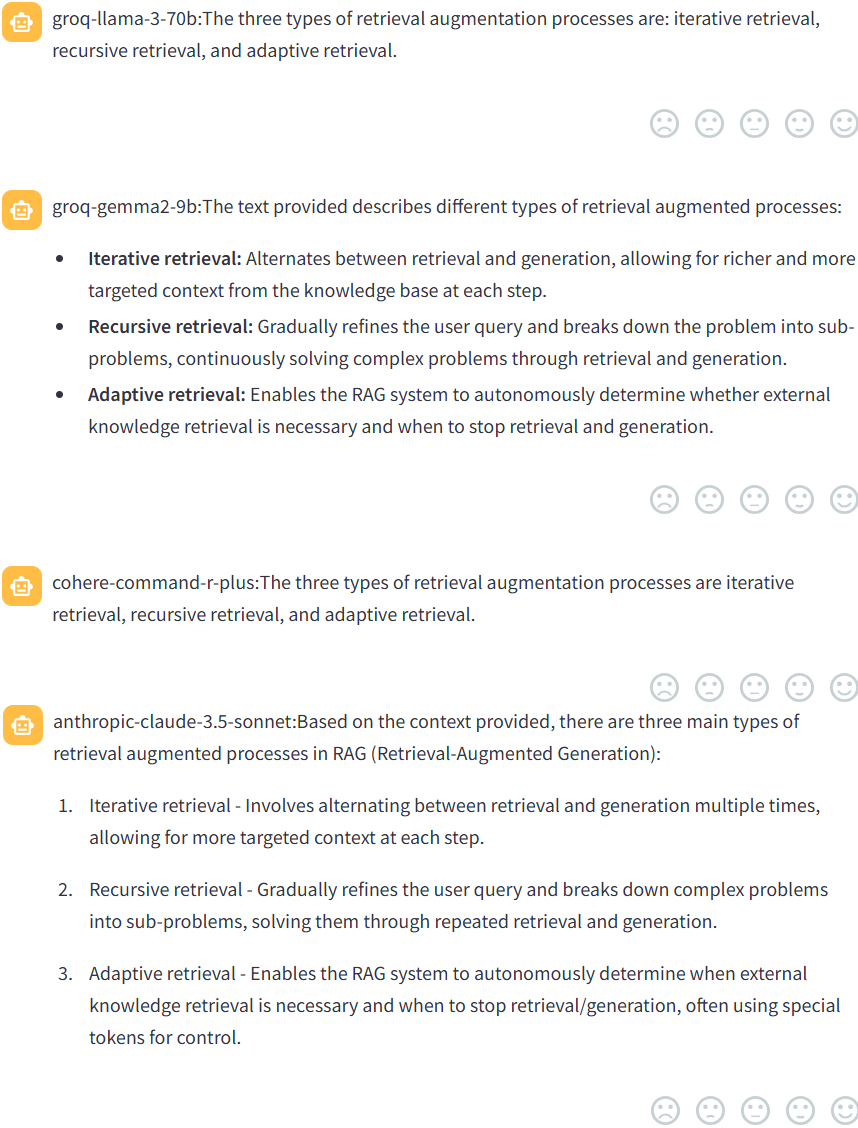
\includegraphics[width=.8\linewidth]{./figures/app-answers.png}
    \caption{Generated answers: not sorted}
\end{figure}
\newpage
We can observe that the generated answers have clear differences. Some models perform better than others in certain cases, and this behavior alternates, meaning it is impossible to determine the best models for every use case. For this example, all the models generated relevant answers, but Claude and Gemma provided further accurate details. The results, however, are not sorted in any order, except the order of which the user has selected their preferred LLMs. It is possible that the more accurate responses get shadowed by less relevant ones (as the case with the Gemma-2 response in this example). Our goal for this app is to allow users to select the LLMs they prefer, while prioritizing better answers first automatically, which can be achieved by checking an option in the web interface to toggle the sorting algorithm.\newline
The following figure demonstrates how the previous answers were sorted to prioritize answers with better quality.\newline
The Gemma-2 and Claude-3.5 models performed better than the other 2 models, providing more information while still sticking to the retrieved context as factual information, while Llama-3 and Command R+ did not use the whole context and returned more succinct answers.\newline
\begin{figure}[htbp]
    \centering
    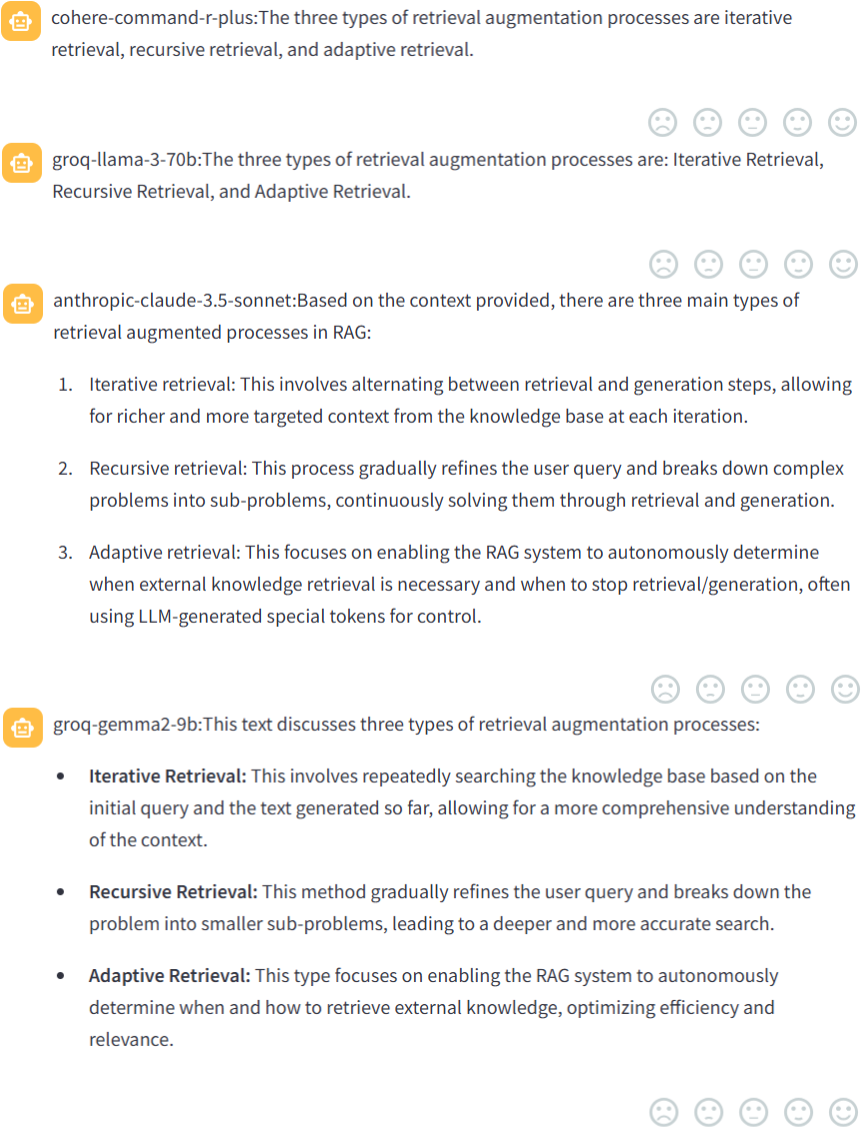
\includegraphics[width=\linewidth]{./figures/app-answers-sorted.png}
    \caption{Generated answers: sorted}
\end{figure}